\begin{figure}
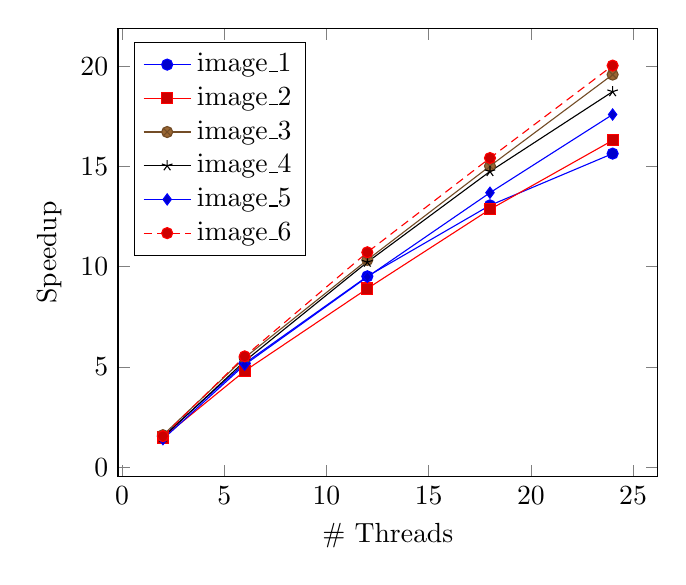
\begin{tikzpicture}
\begin{axis}[legend pos = north west,
xlabel=\# Threads,
ylabel=Speedup]
\addplot+[sharp plot] coordinates {
(2,1.54)
(6,5.18)
(12,9.52)
(18,13.06)
(24,15.64)
};
\addplot+[sharp plot] coordinates{
(2,1.48)
(6,4.80)
(12,8.91)
(18,12.86)
(24,16.30)
};
\addplot+[sharp plot] coordinates{
(2,1.60)
(6,5.46)
(12,10.34)
(18,15.02)
(24,19.58)
};
\addplot+[sharp plot] coordinates{
(2,1.49)
(6,5.29)
(12,10.23)
(18,14.75)
(24,18.73)
};
\addplot+[sharp plot] coordinates{
(2,1.40)
(6,5.11)
(12,9.49)
(18,13.69)
(24,17.59)
};
\addplot+[sharp plot] coordinates{
(2,1.55)
(6,5.53)
(12,10.72)
(18,15.42)
(24,20.03)
};
\legend{image\_1,image\_2,image\_3,image\_4,image\_5,image\_6}
\end{axis}
\end{tikzpicture}
\caption{Speedup for different images and different numbers of threads for local + merge}
\label{linet}
\end{figure}
